\section{Experimental method}

This experiment consists of four parts. First the calibration of the microscope. Secondly size measurements on respectively a human hair, an optical glass fibre and starch particles. Thirdly determining the birefringence of an unknown crystal and finally the computerized improvement of an image of a biological fungus sample. The different experimental methods will be treated separately.\\

The microscope that is used in all experiments is a Leica DM EP microscope. Its manual can be found in appendix \ref{appendix_manual}. This microscope is used in combination with $4\times$, $10\times$, $40\times$ Hi Plan POL objectives with respectfully a 0.10, 0.22 and 0.65 numerical aperture. A color ccd camera in combination with NI Vision Assistant software is used to acquire digital images.\\

\subsection{Calibration}
A microscopic ruler is used to measure the length that corresponds to one pixel in an image. This is achieved by focussing on a 1 mm, 100 division ruler and measuring the distance between two focussed, distant division lines and comparing the number of pixels to the physical length. The NI software is used to find the exact location of these two lines and subsequently find the perpendicular projection (see Figure \ref{fig_pixellength_example}. This procedure is repeated for all three objectives. The relative magnification between two objectives, $M_{A,B}$ can subsequently be found using equation \ref{eq_rel_mag}.

\bigskip

With the aid of a 1951 USAF resolution target, the resolving power of each objective can be found. First taking a focussed grayscale image  on the target and then taking a perpendicular intensity profile for each well defined three-bar structure (see Figure \ref{fig:resolution_target}).This intensity profile is exported by NI Vision to a CSV file directly so we dont suffer from any compression, a file which can be easily read by a python peakfinding script ( an example of which can be seen in the next section's figure \ref{fig:linetrace}). The high and low intensity values will be used to calculate the visibility using equation \ref{eq_visibility} and the corresponding spatial frequency. This is repeated for all three objectives.\\

\subsection{Microscopic size measurements}

All microscopic size measurements are made by measuring pixels and comparing this to the corresponding pixel length. This is done for images with the $40\times$ objective since this gives the smallest error.\\

\subsubsection{Human hair and optical glass fibre}

Measuring the thickness of the human hair and optical glass fibre is done with the aid of the NI Vision software. First finding the two straight lines of the outer edges and subsequently measuring the perpendicular distance between the two. The actual size and error can be calculated using respectfully equation \ref{eq_size_measurement} and \ref{eq_u_size_measurement}.

\subsubsection{Starch particles}

In order to measure the size of individual starch particles, a small amount of starch is mixed with oil. Images are taken at different locations in the mixture. For ellipse-shaped particles that are focussed in the image, an ellipse can manually be fitted.\\

For this experiment it was chosen to find the ellipse size for 30 particles.\\


\subsection{Birefringence}

In order to find the birefringence, $\delta n$, of the unknown crystal, it is placed in the microscope with the polariser crossed with respect to the analyser. The crystal is then turned until bright colours can be seen. Now the path difference, $\delta l$, is measured as a function of the thickness, $D$, of the crystal. $D$ can be found by viewing a border between adjacent colour planes and subsequently noting the focussing position, $f$, of each colour plane. Taking the difference between two values of $f$ will give the difference in thickness, $d$, between two colour planes. The bottom of the sample (black) is also to be taken into account with the same procedure as described above. \\

For this experiment it was chosen to find $D$ and $\delta l$ for 5 colour planes. The focussing process was repeated 4 to 5 times for every border that was studied.\\

\subsection{Image improvement methods}
The features of an image are easier to distinguish when the image has plenty of contrast, an underexposed image might hold a lot of information that is not yet visible for us.\\
A way of qunatitatively expressing the contrast of an image is through a histogram as outlined in the NI Vision article\cite{histogram_theory}. To create such an histogram a python script has been written. Two example files were worked on by the python file, the result of wich is plotted in figures \ref{fig:lcphoto} and \ref{fig:hcphoto}. Both photos have the same pattern on top but a different shade of grey as a background.\\

\begin{figure}[h!]
    \centering
    \begin{minipage}{.5\textwidth}
      \centering
      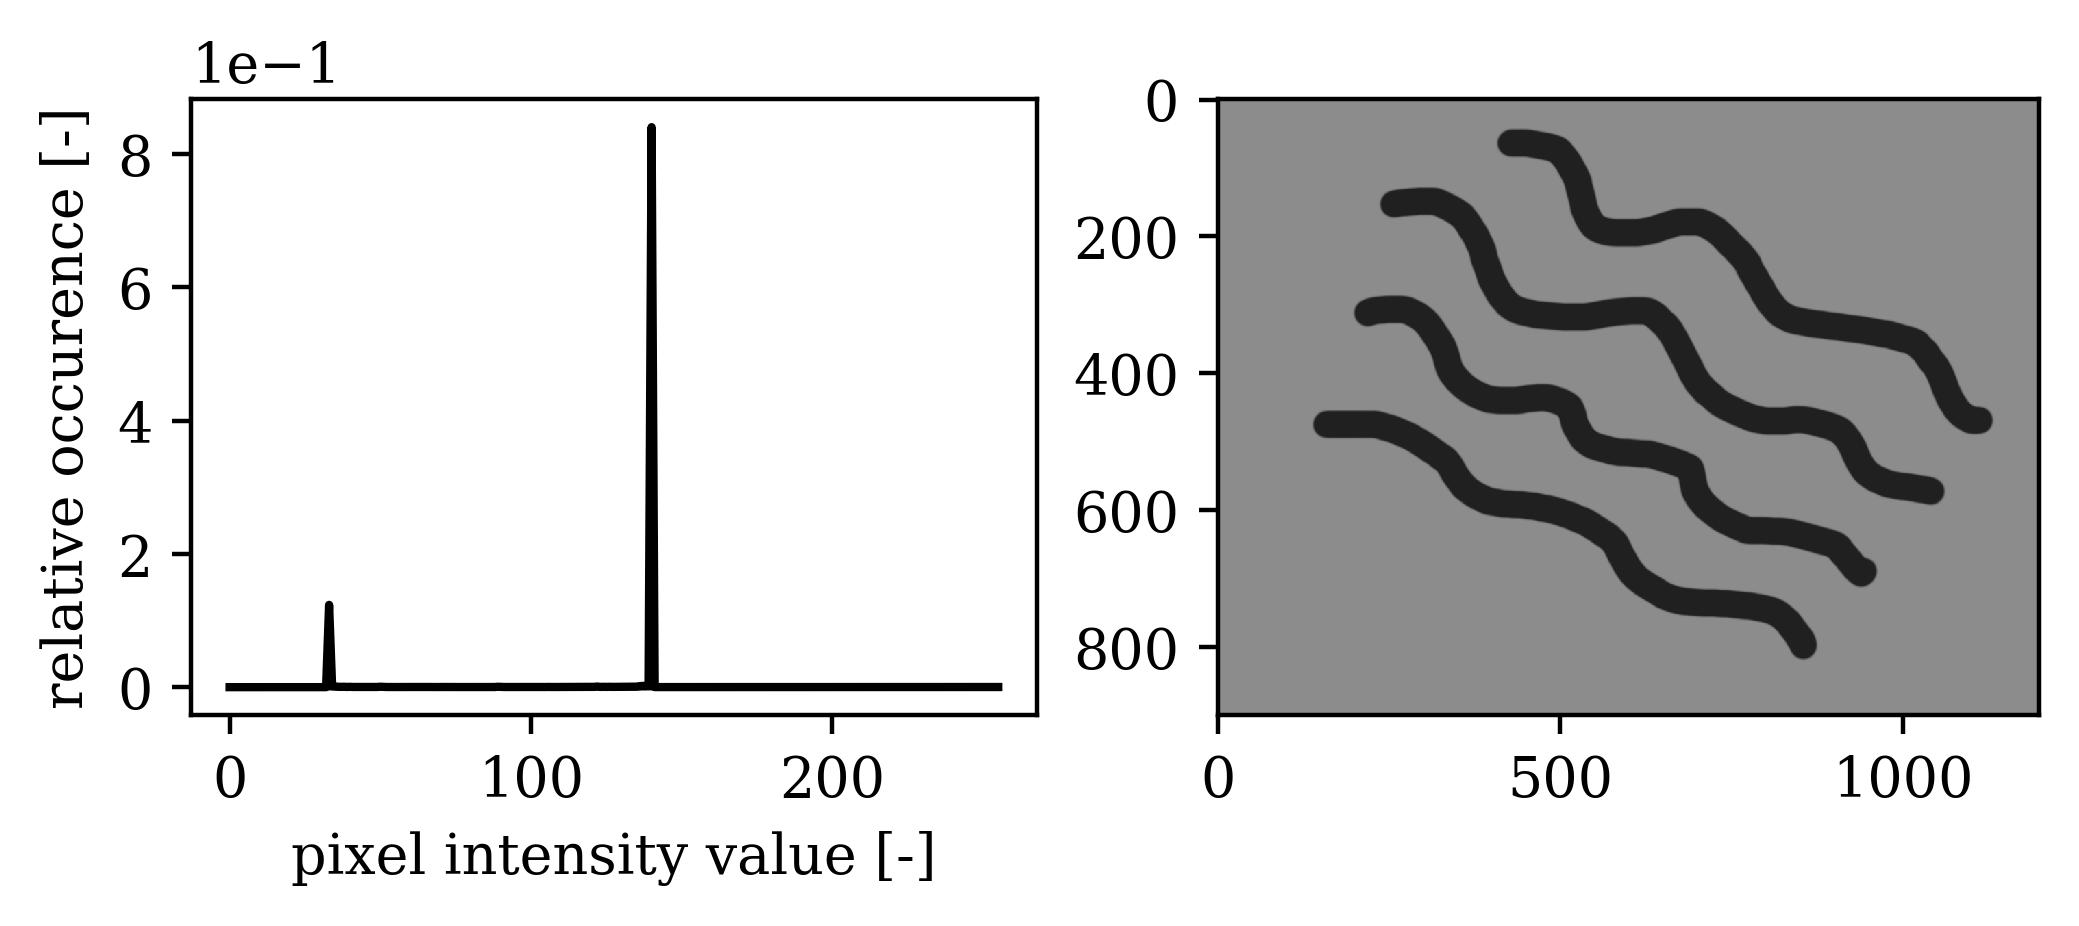
\includegraphics[width=0.9\textwidth,keepaspectratio]{afbeeldingen/histograms/highcontrast.png}
      \caption{High contrast photo}
      \label{fig:hcphoto}
    \end{minipage}%
    \begin{minipage}{.5\textwidth}
      \centering
      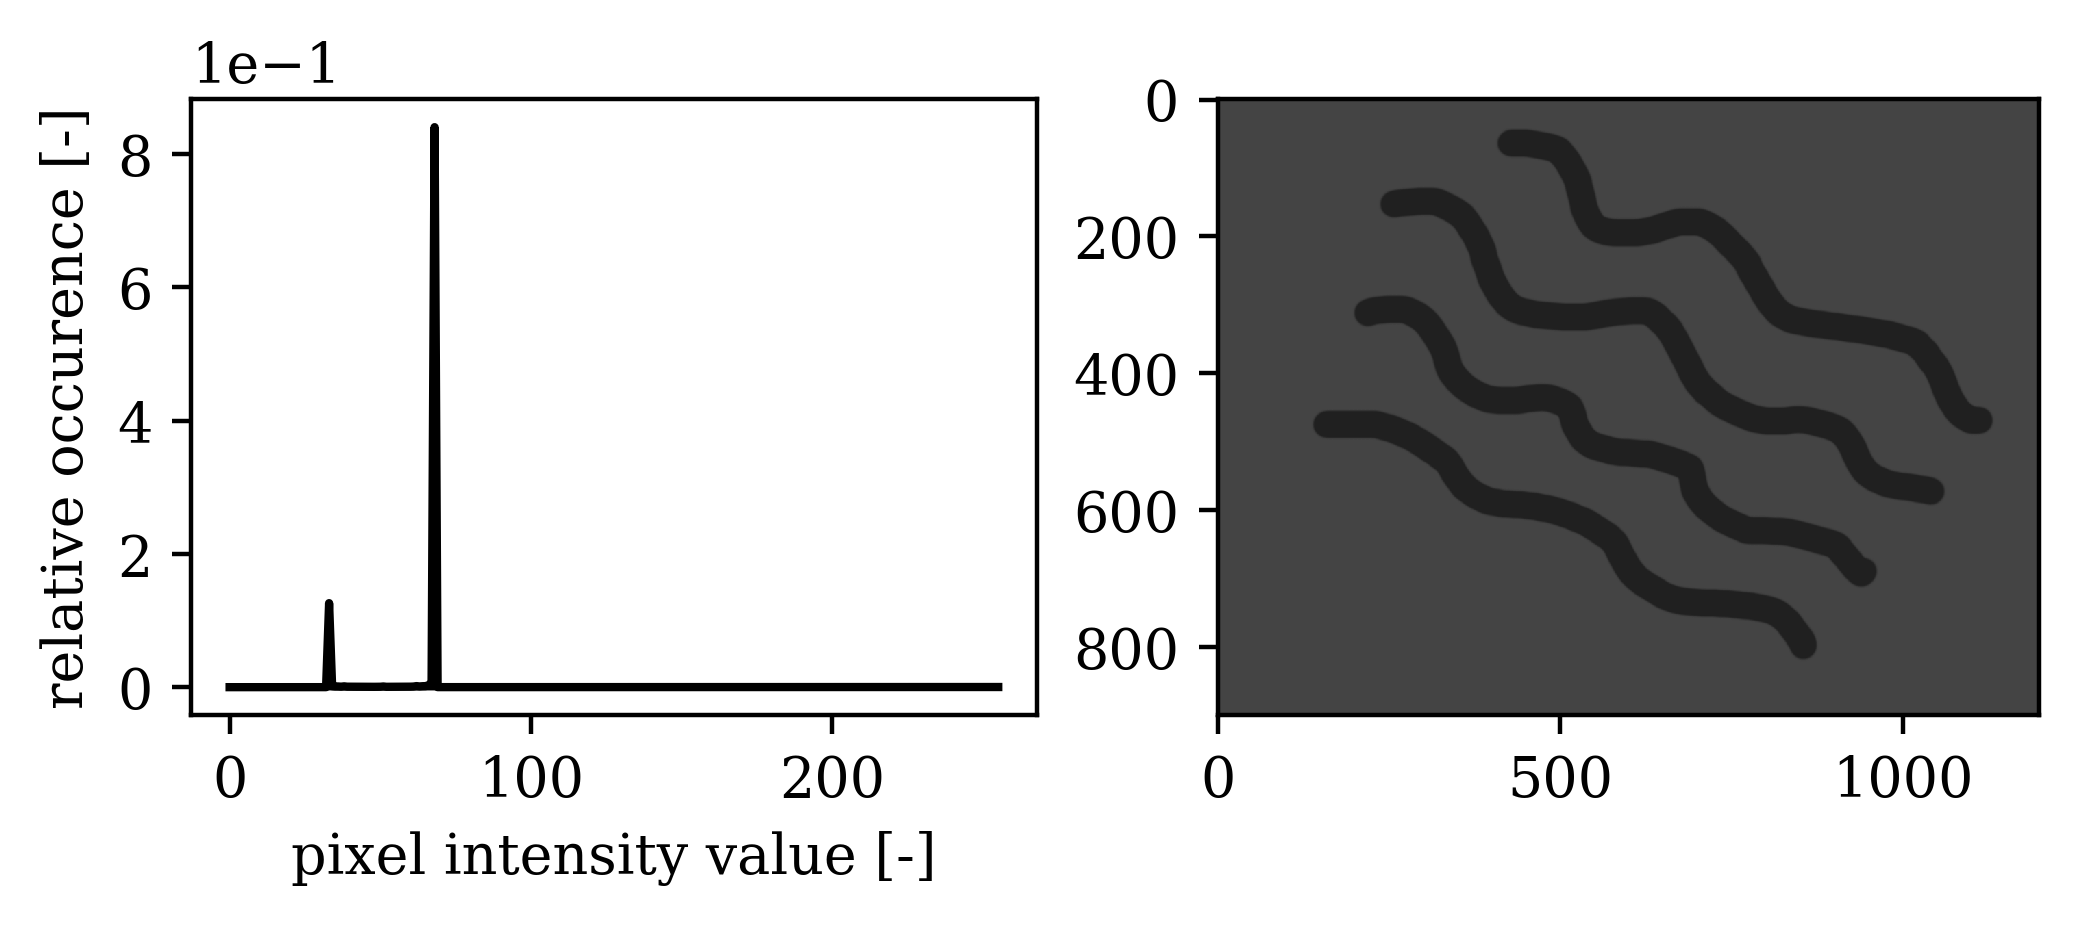
\includegraphics[width=0.9\textwidth,keepaspectratio]{afbeeldingen/histograms/lowcontrast.png}
      \caption{Low contrast photo}
      \label{fig:lcphoto}
    \end{minipage}
\end{figure}

As can be seen in figure \ref{fig:hcphoto} the image has high contrast, the peaks from the squigly lines and the background are seperated in the histogram. Figure \ref{fig:lcphoto} has its peaks closer together meaning that its contrast is lower and thus its features are harder to differentiate from the background.\\
Our goal in this practicum is to devise a way in which we can alter the contrast of a low contrast photo in such a way that it will be easier to distinguish certain features. This method has its drawbacks however since we artificially widen the gap between the peaks which will mean that while we stretch the information between the peaks over a greater intensity range we compress features in the high and low intensity value range.\\
\\
One way of widening the gap between the peaks in the histogram is by applying a sigmoid function on the photo, as sigmoid function is a function $f(x)$ that maps its domain to values between zero and one. This sigmoid equation \ref{eq:sigmoid} depends on two parameters $\alpha$ and $\beta$ wich respectively define the center and the width of the function.

\begin{equation}
    f(x) = \frac{1}{1+e^{-\frac{x-\alpha}{\beta}}}
    \label{eq:sigmoid}
\end{equation}
\newpage
\begin{wrapfigure}{l}{0.55\textwidth}
    \centering
    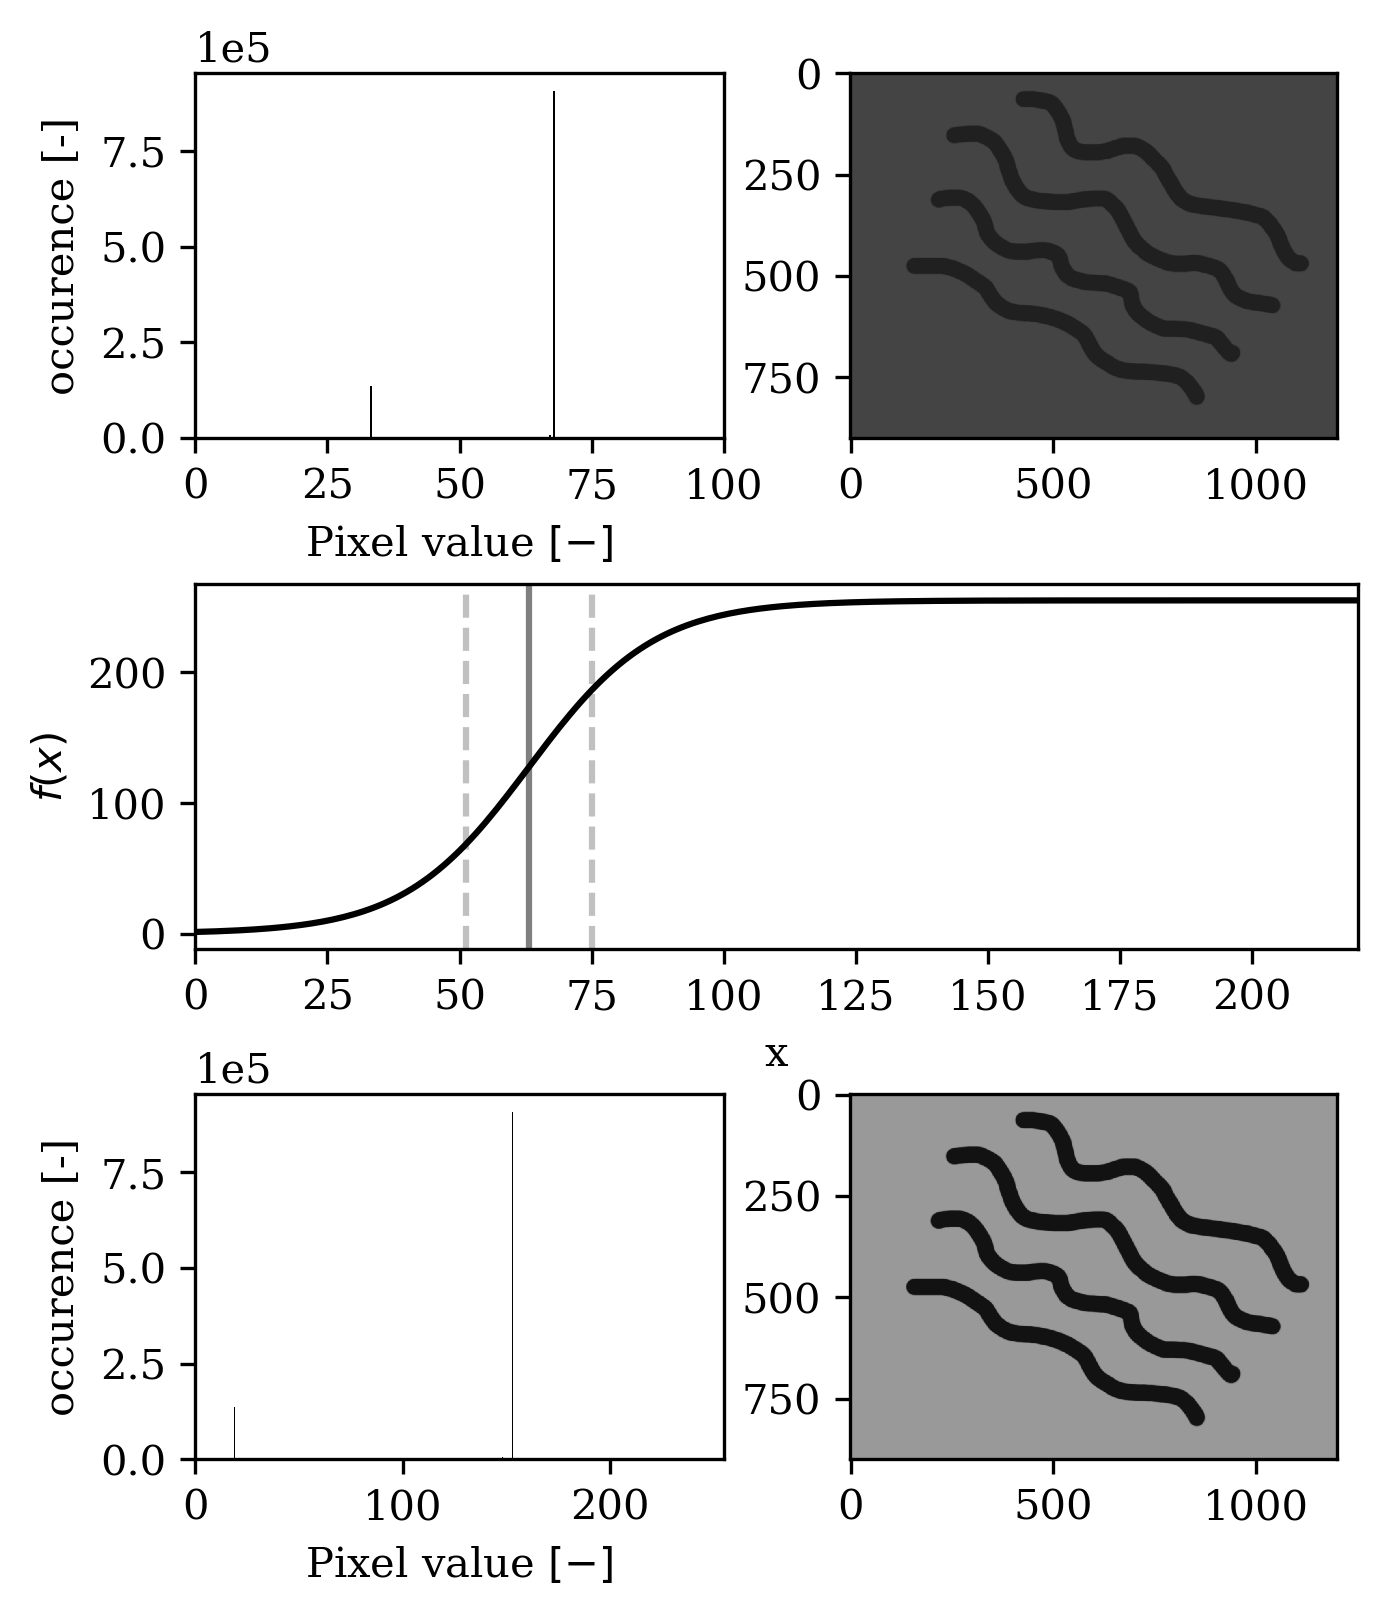
\includegraphics[width=0.55\textwidth,keepaspectratio]{afbeeldingen/sigmoid_explained.png}
    \caption{The example figure modified using a sigmoid function.}
    \label{fig:sigmoid}
\end{wrapfigure}

In figure \ref{fig:sigmoid} on the left the low contrast example figure and its histogram are plotted in the top row, in the middle row a sigmoid function has been plotted as well as the median value and the standard deviation of the histogram above denoted by the grey solid and dashed line respectively. The bottom row consists of the histogram of the example image and the image acted on by the sigmoid function. In this example we used a sigmoid function $f'(x)=f(x) \cdot 255$ since we want to map our input values on a domain $[0,255]$ not $[0,1]$, $\alpha$ is the median of the top histogram and $\beta$ its standard deviation.\\
As can be seen in the figure the peaks of the most common values of the intensity have been spread further apart thus resulting in a higher contrast image.\\






\begin{comment}
The Experimentele opstelling or Experimentele  methode (Experimental  set  up  or  Experimental method) chapter describes the experimental setup and the experimental methods used in sufficient detail such that a reader can judge the soundness and, in principle, may verify the conclusions of your research. Also,  this  chapter  should  be  informative  for  a  reader  who  wants  to  perform  similar  research.  Preferably  use clear sketches of the setup, rather than photographs. In this chapter you also describe the accuracywith which direct observables have been measured, and the accuracy of the important deduced quantities. Detailed accuracy calculations should be put in an Appendix
\end{comment}
